%%%%%%%%%%%%%%%%%%%%%%%%%%%%%%%%%%%%%%%%%%%%%%%%%%%%%%%%%%%%%%%%%%%%%%
%% Copyright waiver
%%%%%%%%%%%%%%%%%%%%%%%%%%%%%%%%%%%%%%%%%%%%%%%%%%%%%%%%%%%%%%%%%%%%%%

\documentclass{beamer}
\usetheme[faculty=econ]{fibeamer}

\usepackage{booktabs}
\usepackage{multirow}
\usepackage[nodayofweek]{datetime}
\usepackage{zed-csp}

\newdateformat{mydate}{\twodigit{\THEDAY}{ }\shortmonthname[\THEMONTH], \THEYEAR}

\makeatletter
\renewcommand\fibeamer@includeLogo[1][]{}
\makeatother

\usepackage[utf8]{inputenc}
\usepackage[main=english, czech]{babel}

\usepackage{ragged2e}
\usepackage{booktabs}
\usepackage{tabularx}
\usepackage{tikz}
\usetikzlibrary{calc, shapes, backgrounds}
\usepackage{amsmath, amssymb}
\usepackage{url}
\usepackage{listings}

\newlength{\myMheight}
\settoheight{\myMheight}{M}

\usepackage{scalerel}

\frenchspacing

\title{Overview of Research and Expertise}
\subtitle{Finance Department, IBSS \\ 
Xi’an Jiaotong-Liverpool University\\\vspace{2cm}}
\author{Wenbin Wu\\ \today}

\begin{document}
\shorthandoff{-}
\frame[c]{\maketitle}

\AtBeginSection[]{%
\begin{frame}<beamer>
\frametitle{Outline}
\tableofcontents[currentsection]
\end{frame}}

\section{Self Introduction}

% Frame for the introduction
\begin{frame}{Self Introduction}
\framesubtitle{Wenbin Wu}
    \begin{itemize}
        \item \textbf{Current Research Focus}
        \begin{itemize}
            \item Computational finance and DeFi using agent-based modeling.
        \end{itemize}

        \item \textbf{Specialization}
        \begin{itemize}
            \item Price stability mechanisms of on-chain collateralized stablecoins.
        \end{itemize}

        \item \textbf{Experience}
        \begin{itemize}
            \item ABM simulation and sensitivity analysis. 
            \item Large scale stylized on-chain data analysis.
            \item Formal verification.
        \end{itemize}
    \end{itemize}
\end{frame}

% Frame for Education background
\begin{frame}{Education}
\framesubtitle{Wenbin Wu}
\begin{itemize}
\item \textbf{King’s College London}
\begin{itemize}
\item PhD in Computer Science
\item MSc Banking and Finance
\end{itemize}

\item \textbf{Peking University}
\begin{itemize}
\item MS Computational Finance
\end{itemize}

\item \textbf{University of Electronic Science and Technology of China}
\begin{itemize}
\item BSc Information Security
\end{itemize}
\end{itemize}
\end{frame}

\section{Current work}

\begin{frame}{PhD Research}
\framesubtitle{Background and Question}

\begin{itemize}
\item \textbf{Background}
\begin{itemize}

\item Stablecoin is a type of decentralized cryptocurrency.
\item Many stablecoins have experienced bank runs. 
\item Some encoutered outright collapse, e.g., Terra 
\includegraphics[height=1.2\myMheight]{resources/terra.png} and Basis 
\includegraphics[height=1.2\myMheight]{resources/basis.jpg}. 
\end{itemize}
\item \textbf{Question}
\begin{itemize}
\item What stablization policies improve price stability?
\item What is the implication of this?
\end{itemize}
\end{itemize}
\end{frame}

\begin{frame}{PhD Research}
\framesubtitle{Methods and Findings}

\begin{itemize}
\item \textbf{Methods}
\begin{itemize}
\item Analysis of stylized blockchain data and smart contracts.
\item ABM simulation. 
\item Some formal verification for the modeled stablecoin system.
\end{itemize}

\item \textbf{Findings}
\begin{itemize}
\item Two key parameters are most notable, \textcolor{red}{collateralization ratio} and \textcolor{red}{auction discount curve}.
\item High collateralization helps reduce irrational runs, and a steep discount curve limits the damage of rational runs. 
\item Runs are inevitable. Many on-chain stablecoins are taking up risky or dubious assets.  
\end{itemize}
\end{itemize}
\end{frame}


\begin{frame}{Collaboration}
\framesubtitle{Professional Collaborations and Roles}
\begin{itemize}
\item \textbf{SoCityDAO and MIT Media Lab}
\begin{itemize}
\item Collaborated with SoCityDAO on carbon credit stablecoin.
\item Assisted in designing their token framework.
\item Advised on blockchain application for carbon credit trading.
\end{itemize}
\item \textbf{School of Economics, Peking University}
\begin{itemize}
\item Assisted in research on the Chinese CBDC under the guidance of a leading economist.
\item Contributed to conference presentations and policy briefs.
\end{itemize}
\end{itemize}
\end{frame}


\section{Future}

\begin{frame}{Highlights}
\begin{itemize}
\item Cryptocurrency and Blockchain Research
\item Interdisciplinary experience intersecting with financial policy
\item Experience with economic experiments on Miner's Dilemma
\item Presenting at various seminars
\item Tools: 
\begin{itemize}
    \item Python and NetLogo for ABM
    \item Python (joblib for multip), R, and SQL for financial statistics
    \item Solidity, Infura, and Web3 for blockchain integration
\end{itemize}
% \item Simple spatial SIR model
% \item Some understanding in 3D physics (game engines) 
\end{itemize}
\end{frame}



%     \begin{frame}{If I were to partake the project}
%   \begin{itemize}
%       \item \textbf{Collaboration}: Bridge AI and Net Zero challenges, enhancing team synergy.
%       \item \textbf{Data Fusion}: Automate model rescaling for accurate climate-based projections.
%       \item \textbf{AI Integration}: Combine machine learning with environmental models.
%       \item \textbf{Communication}: Relay technical findings to diverse teams.
%       \item \textbf{Research Dissemination}: Share results via journals and conferences.
%       \item \textbf{Adaptation}: Delve into spatial statistical models for project advancement.
%   \end{itemize}
% \end{frame}

% \begin{frame}{If I were to partake in the research}
% % \framesubtitle{Some ideas}
% \begin{itemize}
%     \item Initialize spatial space using topologicpy
%     \item Survey airborne transmission dynamics (Riley 1978, Riley 2011)
%     \item Combine the two to initialize the spread of infectious dose
%     \item Intervention parameters and their reduction of infectious dose
%     \item Consider agent movement, infection, and evaluation
% \end{itemize}
% \end{frame}

\begin{frame}{Thank you}

\end{frame}

\begin{frame}{Appendix: Some Stylized Data}
\begin{figure}
\centering
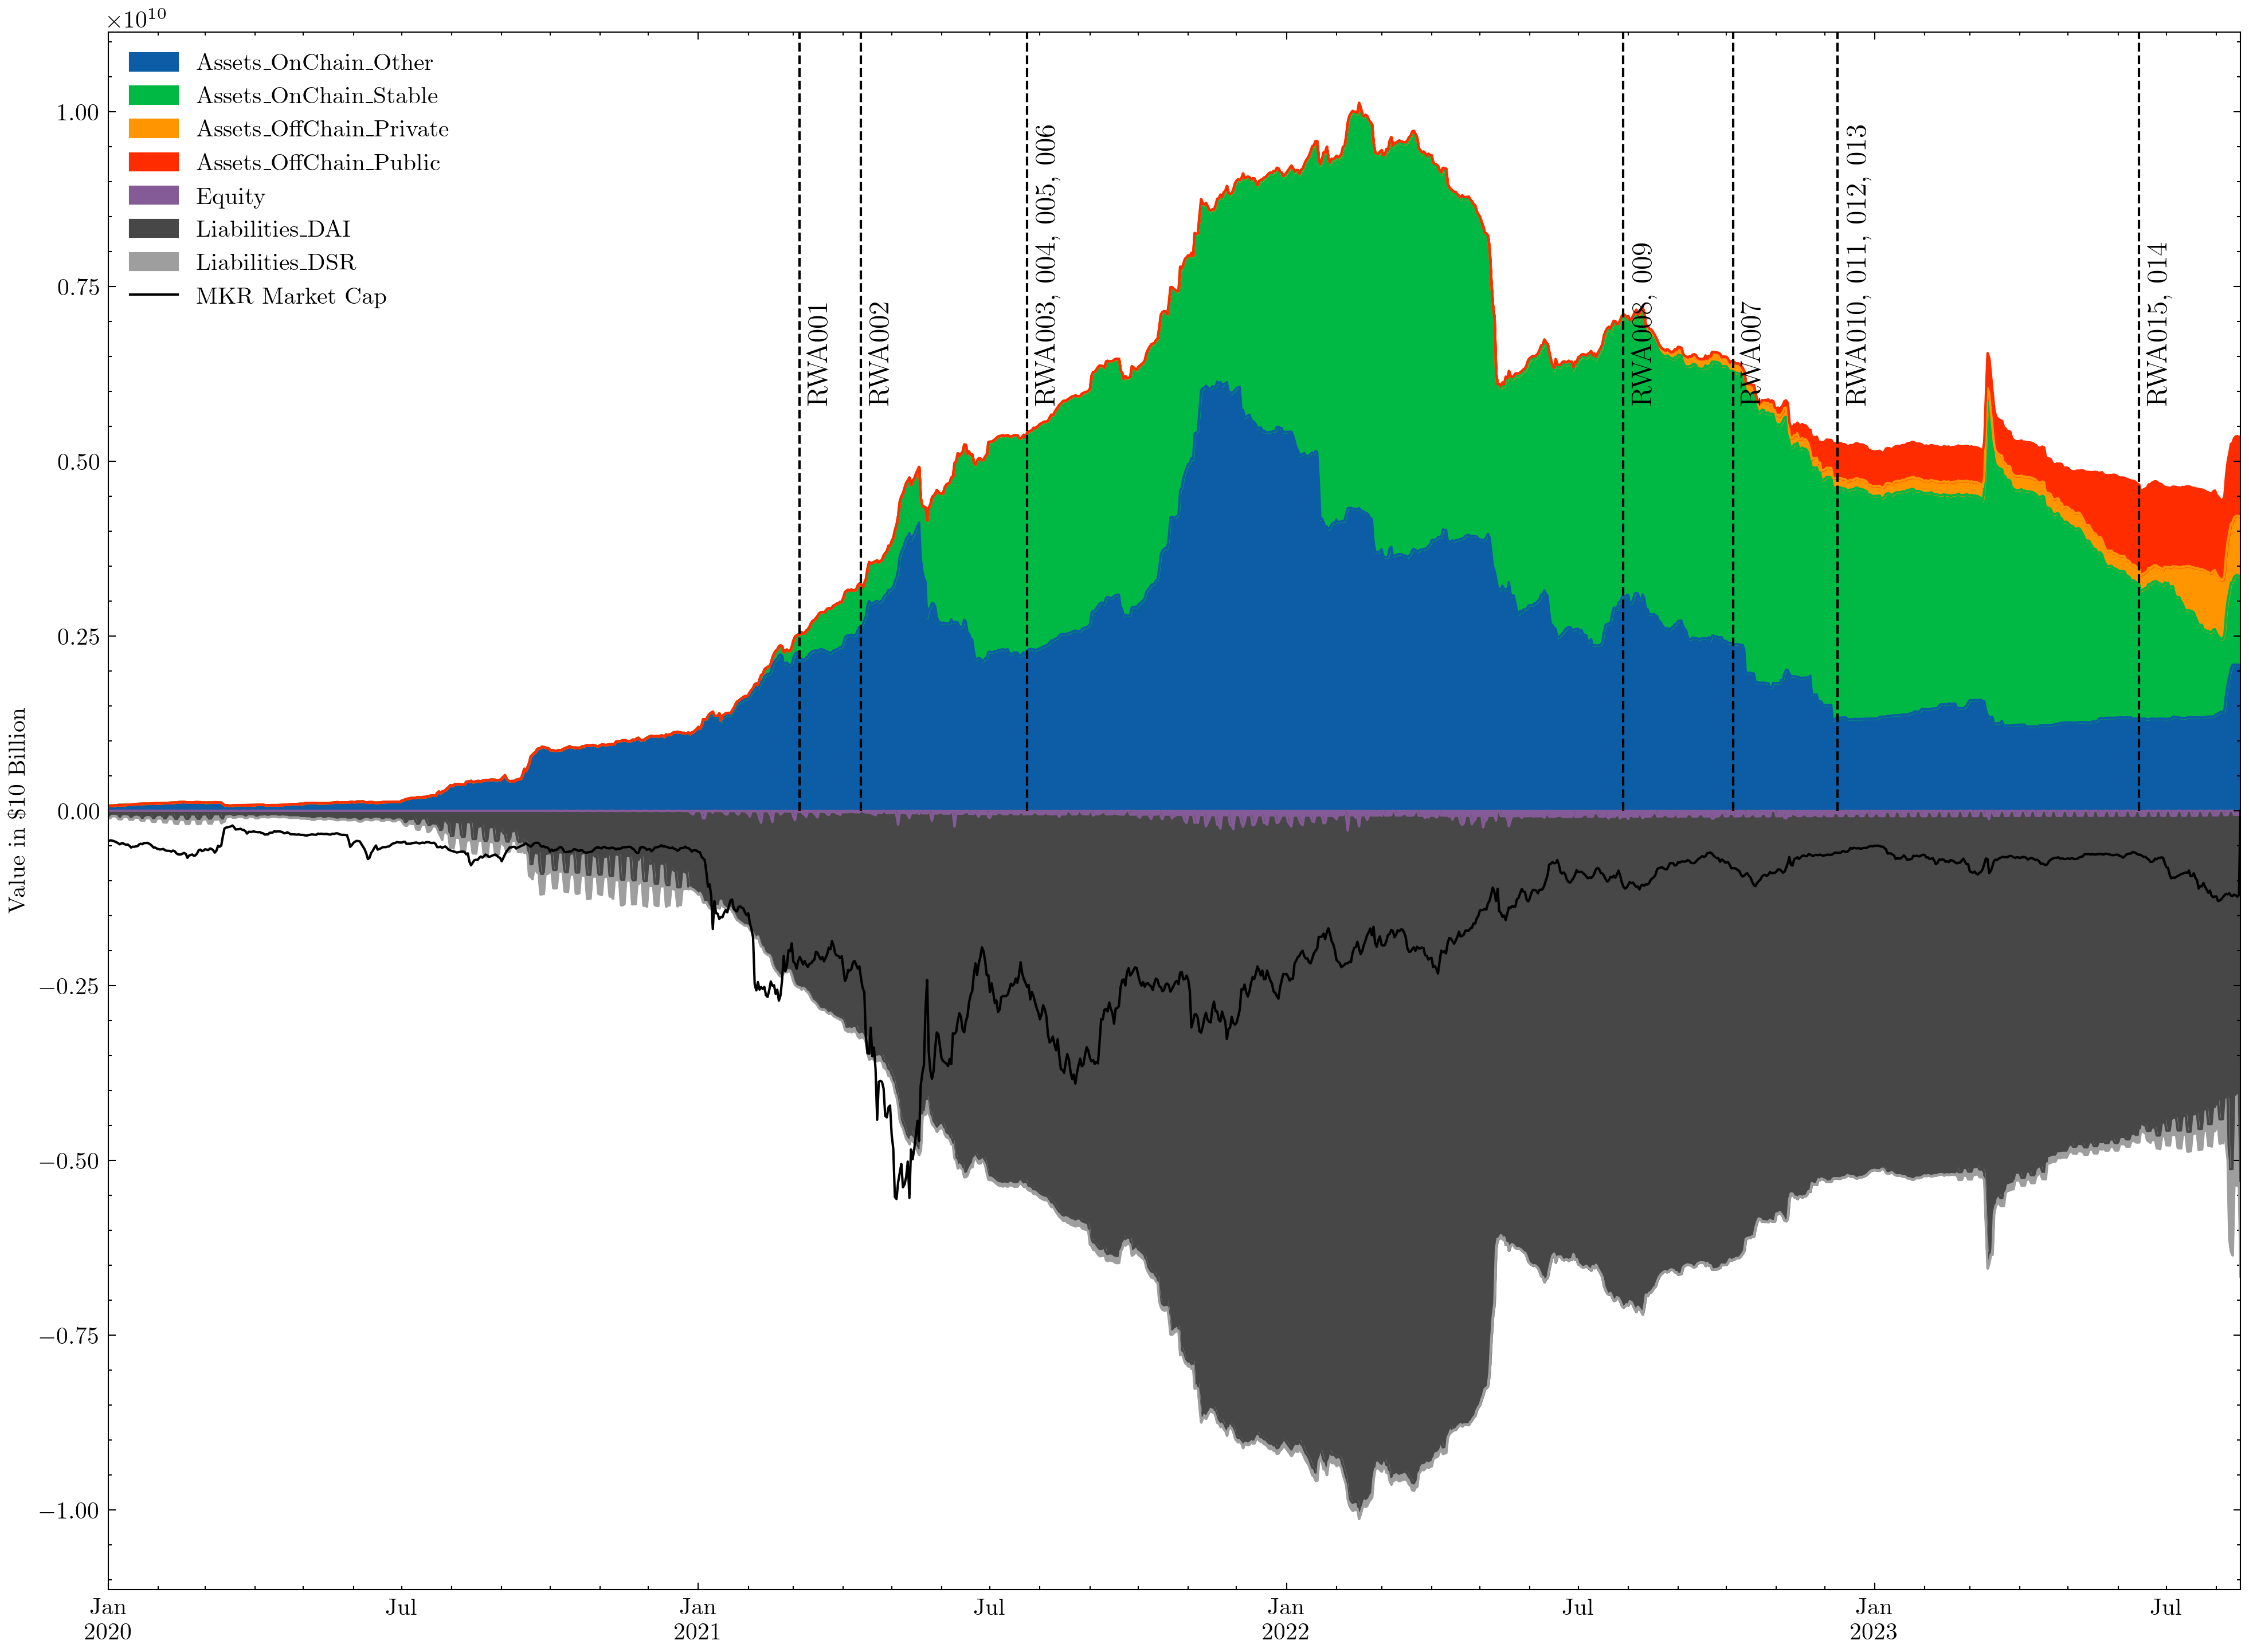
\includegraphics[width=90mm]{Figs/historical_balancesheet_with_votes.png}
\caption{MakerDAO Balance Sheet, 2020-2023}
\label{fig1}
\end{figure}
\end{frame}

\begin{frame}{Appendix: Some System Components}
\begin{figure}
\centering
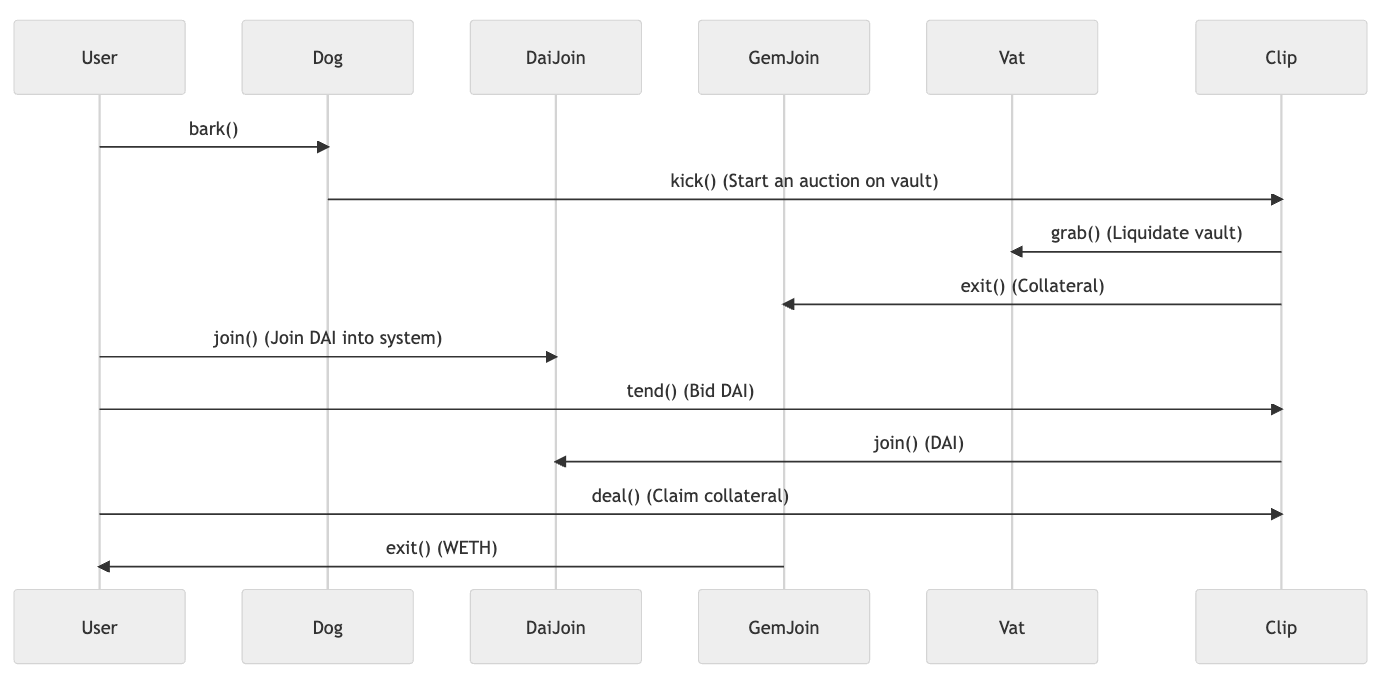
\includegraphics[width=100mm]{resources/system.png}
\caption{Simplified System Components of MakerDAO}
\label{fig2}
\end{figure}
\end{frame}

\begin{frame}{Appendix: Formal Design of Method}
\begin{schema}{Kick}
\Delta Clipper \\
tab: \real \\
lot: \real \\
% usr: USER \\
kpr: \seq CHAR \\
now: \nat \\
\where
tab > 0 \\
lot > 0 \\
kicks' = kicks + 1 \\
ACTIVE' = active \cup \{kicks'\} \\
\end{schema}

% \vspace{1cm}  % Add some space between the schema and the caption
\centering
\normalsize{Schema: Begin Collateral Auction}
\vfill  % Fill the remaining space to push the caption towards the bottom
\end{frame}


\begin{frame}{Appendix: Global Interactive Sensitivity}
\begin{figure}
\centering
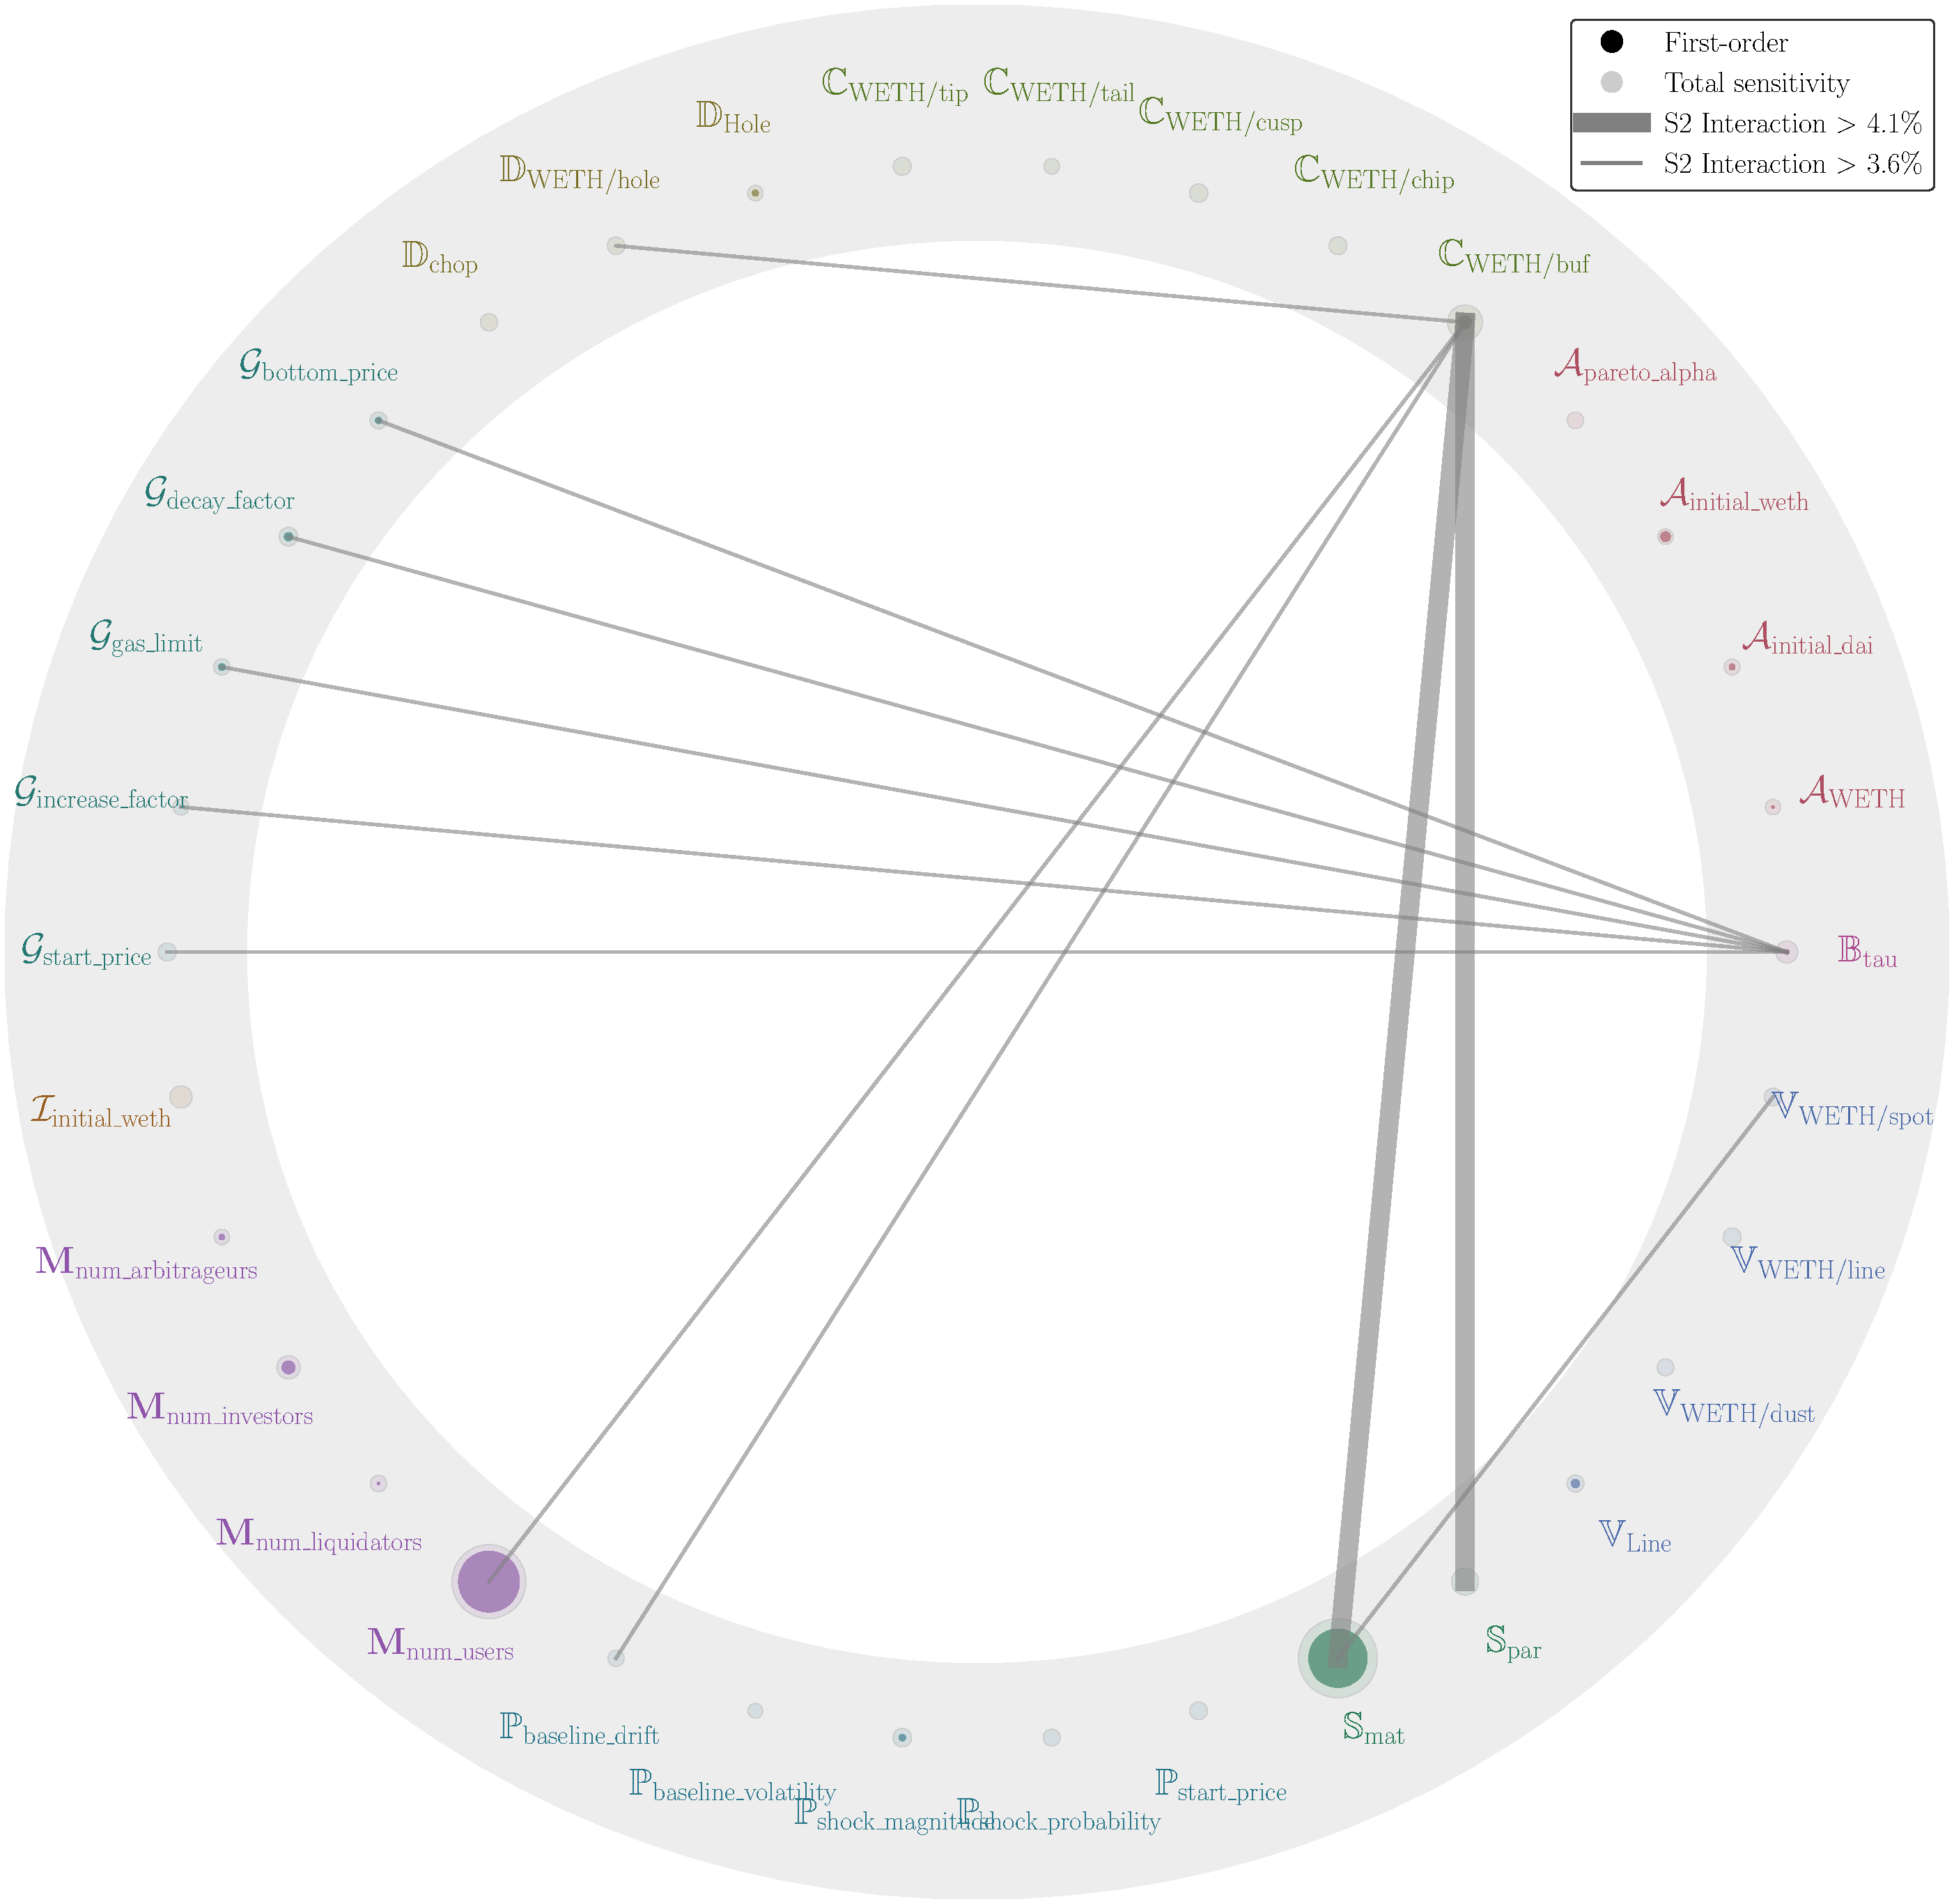
\includegraphics[width=70mm]{Figs/Sobol' Sensitivity Analysis, 35840 model runs.pdf}
\caption{Global Interactive Sensitivity, 35840 model runs}
\label{fig3}
\end{figure}
\end{frame}

\begin{frame}{Appendix: Time series Sensitivity}
\begin{figure}
\centering
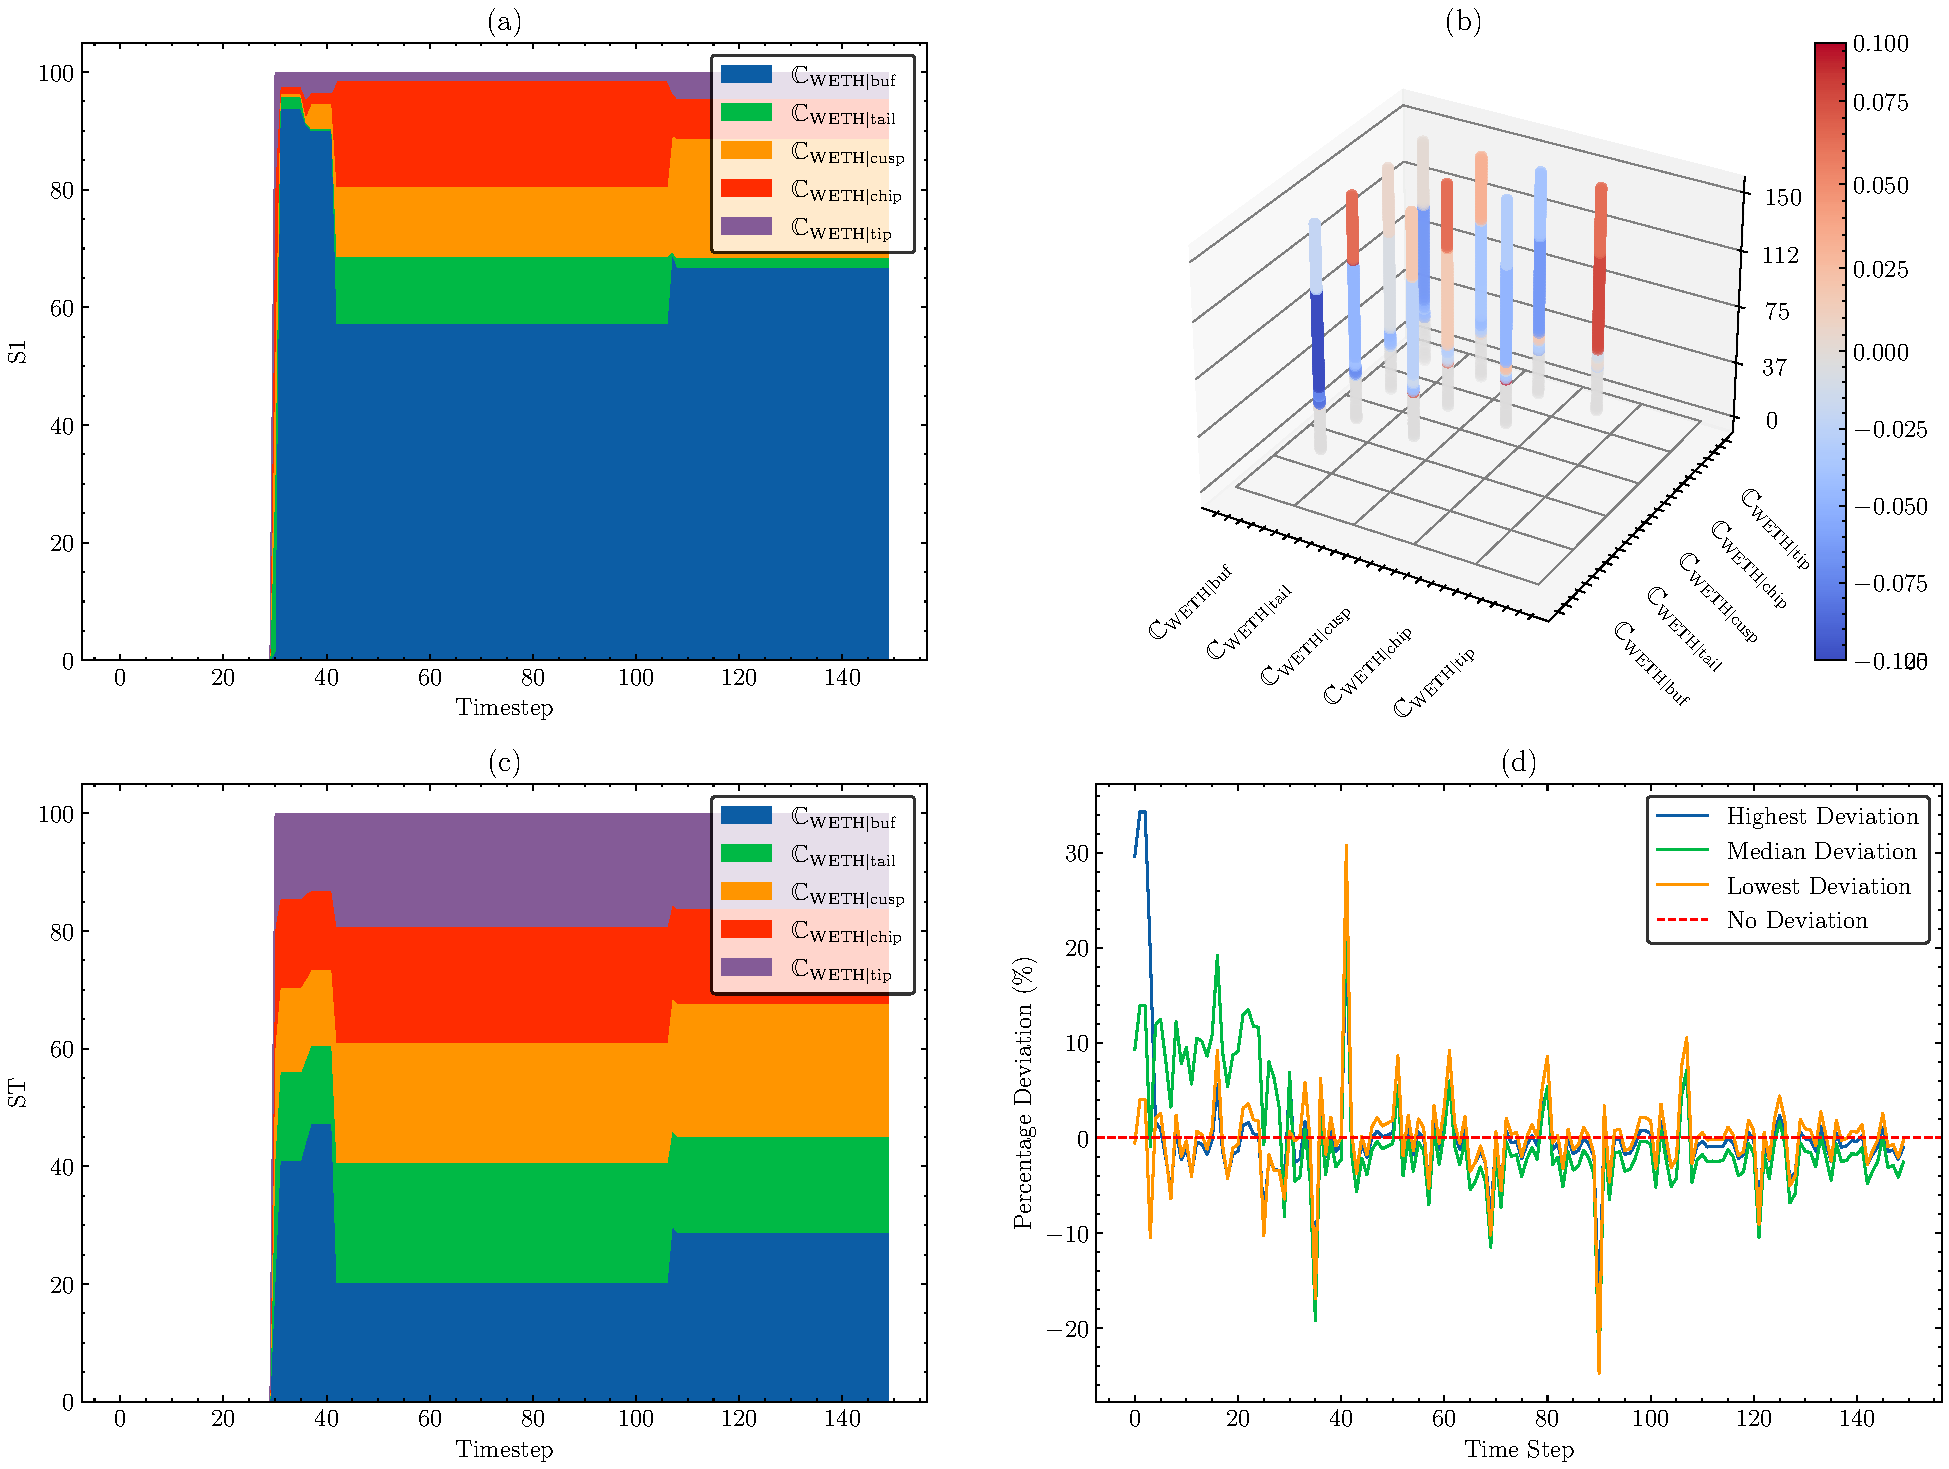
\includegraphics[width=85mm]{Figs/SOBOL_time_series_for_problem_cliplike_n10.pdf}
\caption{Sensitivity Analysis for Auction Parameters, 10240 Model Runs}
\label{fig4}
\end{figure}
\end{frame}


\end{document}
